\chapter{Mathematical Background\index{Mathematical Background}}

\textsf{ In this chapter we provide the mathematical proofs which form the basis
of the prediction models. The main concept of matrix factorization is explained
mathematically. Singular value decomposition is explained in detail, and some
issues regarding the disadvantages in the present scenario is explained. An
substitute method Alternate Least Squares is explained. And lastly low rank
approximation is explained.}

\section{Least Squares and Orthogonality}
\subsection{Linear Systems}
The nature of the problem and the data we are dealing with is linear in nature,
and hence we should start by looking into the basic principles involved in
solutions of linear systems. Almost all the complex linear problems when broken
down to the most granular level, can be viewed as,
\begin{equation} 
  Ax=b,
\label{eq:4.1}  
\end{equation}
where $A\in\mathbb{R}^{m \times	 n}$, $x\in \mathbb{R}^n$ and $b\in
\mathbb{R}^m$. It
is applied to deal with real life problems, by considering $x$ to be vector of
causes and $b$ to be the vector of effects of a system which is characterized by
matrix $A$. So when we know the causal vector $x$ we can find the effect $b$, by
$b=Ax$. Or in most data modeling problems, we know the effects(from the
\emph{training data}), $b$, we need to find the causal vector $x$. 

If $m=n$, $A$ happens to be square and it is
expected to be nonsingluar in order to have a unique non-trivial solution. Here
the vector $b$ can be represented as a linear combination of the columns of $A$.
This simply means that $b\in span(A)$, where $span(A)={Ax:x\in \mathbb{R}^n}$ 

However not all problems in real life is as simple as this, we have to deal with
rectangular sytems, i.e., $m\neq n$. Well on most scenarios when this happens,
we have $m\geq n$, and we have different iterative approaches to its solution. 
\subsection{Vector and Matrix Norms}
Since we will be approximating the unknown vectors and eventually matrices, we
need to have way to measure their 'sizes'. Hence we need to apply the scalar
concepts of, magnitude, absolute value, or modulus to vectors and matrices.

We can measure the 'size' of vectors by,
\[
 {\|x\|}_1 = \sum_{i=1}^{n}|x_i|,		1-norm,
\]

\[
 {\|x\|}_2 = \sqrt{\sum_{i=1}^{n}x_i^2},		2-norm,
\]

\[
 {\|x\|}_\infty = \sum_{i=1}^{n}|x_i|,		max-norm,
\]
 In a generalized form, the \emph{p-norm} is defined as, 
 \[
 {\|x\|}_2 = \sqrt[p]{\sum_{i=1}^{n}x_i^p}
 \]

 The matrix norms for matrix $A\in\mathbb{R}^{m \times n}$as computed as
follows,
 \[
 {\|A\|}_1 = \underset{1\leq j\leq n}{max}{\sum_{i=1}^{m}|a_{ij}|}
 \]
 \[
 {\|A\|}_2 = (\underset{1\leq j\leq n}{max}{\lambda_i(A^TA)})^{1/2}
 \]
Our main goal in this thesis work is to approximate a matrix by predicting the
missing values. In order to do this we minimize the residual, $r$, between the
known rating matrix $R\in\mathbb{R}^{m \times n}$ and the approximating matrix
$\hat{R}\in\mathbb{R}^{m \times n}$. While finding the residual, we treat the
two matrices, $R$ and $\hat{R}$ as points in $\mathbb{R}^{mn \times mn}$, and we
use a special \emph{Frobenius norm}, to calculate the distance between them,
 \[
 {\|A\|}_F = \sqrt{\sum_{i=1}^{m}\sum_{j=1}^{n}a_{ij}^2}.
 \]
 
 \subsection{Bases and Rank of Matrix}
 Suppose we are dealing with a real space, $\mathbb{R}^m$, it is handy
to have a fixed number of vectors, making use of which we can span the entire
space under consideration. This collection of fixed number of vectors is called
\emph{basis} in $\mathbb{R}^m$. 

Let us consider a set of vectors $(v)_{j=1}^n$ in $\mathbb{R}^m$, $m\geq n$, 
\[
 span(v_1,v_2,...,v_n)=\left\{ y|y=\sum_{j=1}^{n}\alpha_{j}v_j \right\}
\]
for arbitrary coefficients $\alpha_j$. The vectors $(v)_{j=1}^n$ are
\emph{linearly independent} when
\[
 \sum_{j=1}^{n}=0 \ iff \alpha_j = 0 for j=1,2,...n.
\]
The maximum number of linearly independent vectors(column or row), is called the
\emph{rank} of the matrix \cite{eld-mm:07}

\subsection{Least Squares}
In almost all problems in which numerical techniques are used to find
solutions, we have to deal with \emph{overdetermined} system, 
\[
 Ax\cong b,
\]
where $A\in \mathbb{R}^{m \times n}$, with $m>n$, $x\in \mathbb{R}^n$ and $b\in
\mathbb{R}^m$. In this case it would not be possible to represent
$m$-dimensional $b$, as linear combinations of only $n$ column vectors of $A$.
It so happens that the points on the LHS and RHS, are not in a common space.
Hence we would look to minimize some norm of the \emph{residual}, $r=b-Ax$. The
solution obtained here is in the \emph{least squares} sense. 


Let us classify the problems, as type-I, in which we have to deal with exactly
or very linearly dependent vectors, and secondly, type-II, in which the system
consists of almost linearly dependent vectors as well. Direct linear solvers
like Gaussian elimination can be applied to type-I problems only. To deal with
type-II, which usually has noise in it, we need to filter out the bad basis
vectors, which are represented by the almost linearly dependent vectors. In
order to quantize the difference between the \emph{very} and \emph{almost}
linear dependence, we make use of orthogonality. The good vectors, i.e., the
very linearly dependent vectors are close to orthogonal. 

\subsection{Orthogonality}
Why is \emph{orthogonality} important to us? Our basic approach in building the
prediction model, is to factorize the rating matrix $R\in \mathbb{R}^{m \times
n}$ with $m>n$, into $P\in \mathbb{R}^{m \times k}$ and $Q\in \mathbb{R}^{n
\times k}$, where generally $k<<n<m$. By reducing the dimensions, we are
removing the bad basis vectors, i.e., vectors carrying no significant useful
information. It is strongly desired that the remaining good basis vectors be
orthogonal to each other. 

Two nonzero vectors $x$ and $y$ are orthogonal to each other, if $x^Ty=0$, which
is the same as $cos\theta=0$, where $\theta$ is the angle between $x$ and $y$. 
\begin{proposition}
Let $q_j$, j=1,2,...,n, be orthogonal, i.e., $q_i^Tq_j=0$, i\unequal j. Then the
vectors $q_j$ are all linearly independent.
\end{proposition}

We will now see how we can decompose the matrix to more compact forms, using
orthogonal transformations. QR decomposition is one stable technique to achieve
this. QR decomposition is not very useful for our problem due to various
reasons, which will me mentioned later, it helps in understanding the concepts
and gradually take us to the more complex methods like SVD, which will be
introduced later. The matrix $A\in \mathbb{R}^{m\times n}$, which is usually the
data matrix, can be factorized as shown below,
\[
 A = Q\left(\begin{array}{ccc}
		R \\
               0  \end{array}\right), 
\]	
where $Q \in \mathbb{R}^{m \times m}$ is orthogonal and $R \in \mathbb{R}^{m
\times n}$ is upper triangular. 

The main reason to factorize the data matrix are, 
\begin{enumerate}
 \item Compact representation
 \item Representation in terms of \emph{basis} in column-space, row-space or
both column and row space. 
\end{enumerate}

Below Figure ~\ref{fig:QR Factorization}, show how QR factorization achieves the
above goals, i.e., firstly compact representation, which is achieved by reducing
the \emph{rank}$=k$. It can be shown that by optimally choosing the rank k, we
get better performance. 
This value of k, can be chosen by trial and error methods. Secondly, QR
factorization helps us in representing the matrix in terms of the basis vectors
in the column space or in the row space. In the figure below, we can see that
the matrix \emph{Q}, forms the orthonormal basis for the column space of
\emph{A}. This means that, the factors in the column space if \emph{A} defines
or characterizes the system. This means that the known information is used only
from only one dimension. So this technique is more suitable for solving linear
systems in least squares sense, as in Equation ~\ref{eq:4.1}, where only the
column-space is sufficient, as the known vector \emph{b} lies in the column
space. 
\begin{figure}[h!]

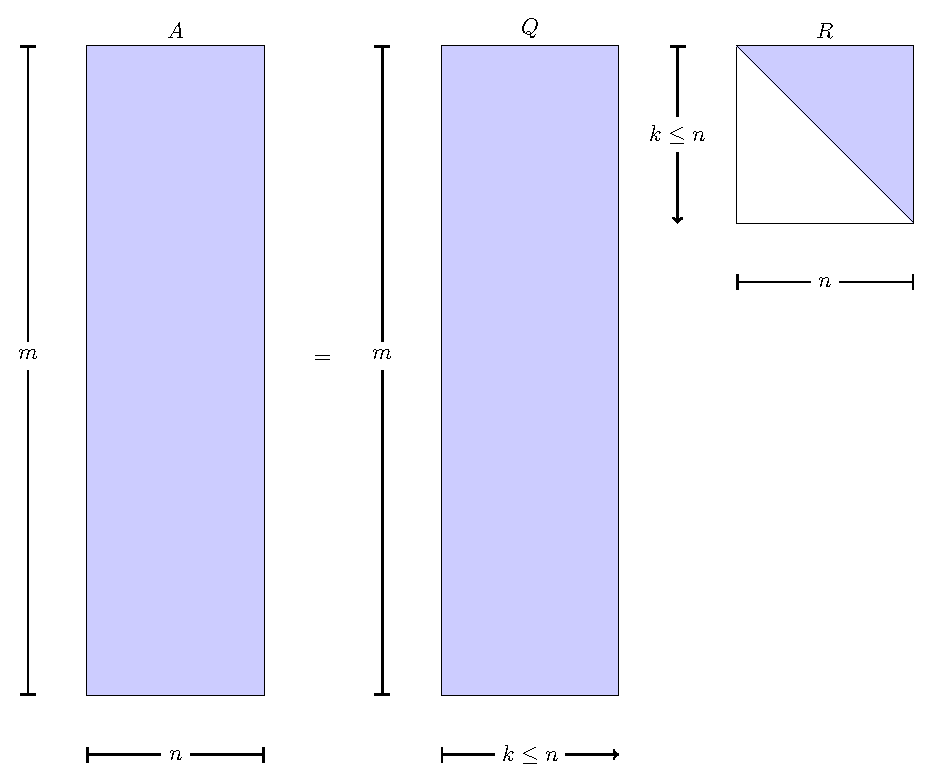
\includegraphics[width=0.9\textwidth]{QR_Fig.pdf}
\caption{QR Factorization with reduced rank, $k$}
\label{fig:QR Factorization}
\end{figure}


We shall consider an example application, to study the concepts discussed. This
example is obtained from \cite{eld-mm:07}. 
\begin{example}
 Consider a text mining application, where we need to search for documents based
on some queries. The documents are listed below, with the keywords highlighted. 

\end{example}


\section{Introduction to Matrix Factorization}
Since this chapter is dedicated to the mathematical principles that drives the
prediction models, we can begin with a direct statement, the data matrix is
factorized into simpler matrices which are constrained on its dimensionality.
Different types of constraints can be imposed on the factorization, but for the
particular machine learning task of collaborative filtering we have only used
the low rank approximation. Collaborative filtering can be considered as
\emph{matrix completion} problem, where we are trying to fill in the missing
entries of the sparsely filled rating matrix $R$ $\in\mathbb{R}^{u,i}$. We
complete the rating matrix by approximating it to a full matrix $\hat{R}=PQ'$,
where $P \in\mathbb{R}^{u,k}$ and $Q \in\mathbb{R}^{i,k}$. 

$P$ and $Q$ are unconstranied \emph{factor matrices} and we will show that if
$\hat{R}$ is the best approximation of the original rating matrix, then the
\emph{rank} of $\hat{R}$ is at most $k$. 

Now that we have had a fair idea of how to approach the problem, the next
important concern is to decide in what sense do we want to approximate the data
matrix, or how do we measure the discrepency between the original matrix and the
approximated matrix. The simplest way would be to measure the \emph{Frobenius
distance} between the two,
\[
 \|{R-\hat{R}}\|_{F}^2 = \sum_{ui}^{}(R_{ui}-\hat{R}_{ui})^2
\]
But we use the Root Mean Squared Error(RMSE) to measure the accuracy. 

There might also be a necessity in applicatons like clustering to impose a
constraint on the factored matrices other than only on rank of approximating
matrix. Since clustering is based on some kind of distance measure and distance
can never be negative, it is obvious that we need to impose a non-negative
constraint on the factored matrices. In such cases we cannot rely on SVD as it
can generate negative elements. Instead we might want to compute the rank-$k$
approximation in the following way \cite{eld-mm:07}, \\
\[
  A\approx WH,		W,H\geq0
\] \\

\section{Matrix approximation using SVD}
\begin{theorem}[SVD]
 Any $m \times n$ matrix A with rank k, with $m \geq n$, can be factorized \\
\begin{equation}
  A = U\begin{pmatrix}\Sigma\\0\end{pmatrix}V^{T},
\end{equation}
where $U \in \mathbb{R}^{m \times m}$ and $V \in \mathbb{R}^{n \times n}$, and
$\Sigma \in \mathbb{R}^{m \times n}$ is a diagonal matrix, i.e., $\Sigma =
diag(\sigma_1,\sigma_2,...\sigma_n)$, with $\sigma_1 \geq \sigma_2 \geq ... \geq
\sigma_n \geq 0$. Here $\sigma_1,...,\sigma_n$ are called singular values of A.
The column vectors of U and V are called the right and left singular vectors of
A, respectivley.  
\end{theorem}
The matrix A can be constructed from the singular values as shown below, \\
\begin{equation}
 A=\sum_{i=1}^{n}\sigma_i u_i v_i^T
\end{equation}
The matrix $U$ can be written as $U=[U_1 U_2]$, where $U_1 \in \mathbb{R}^{m
\times n}$. We can obtain the matrix $A$ by the \emph{outer} \emph{product}
\emph{form} in a thin version as shown below,
\[
 A=U_1 \Sigma V^T = \begin{pmatrix}u_1&u_2&\cdots&u_n\end{pmatrix}
  \begin{pmatrix}
  \sigma_1 &         &        &        \\
           & \sigma_2&        &        \\
           &         & \ddots &        \\
           &         &        & \sigma_n
 \end{pmatrix}
 \begin{pmatrix}v_1^T\\v_2^T\\\vdots\\v_n^T\end{pmatrix}\\
\] \\
Now moving ahead with matrix approximation, let us consider our original matrix
$A$, as sum of a low-rank matrix and a small noise, $A_0 + N$. Since it is an
approximation problem we will try to minimise the noise $N$, by estimating the
\emph{correct rank} of $A_0$, this rank is known as \emph{numerical rank}.
\cite{eld-mm:07}. Now the approximation looks like this, \\
\[
 A = \sum_{i=1}^{n}\sigma_i u_i v_i^T \approx \sum_{i=1}^{k}\sigma_k u_k v_k^T
\]\\
\begin{theorem}[Eckart-Young theorem]
 For a matrix A $\in \mathbb{R}^{m \times n}$, with $rank(A)=r>k$. The Frobenius
norm of the matrix approximation problem \\
\begin{equation}
 \min_{rank(\hat{A})=k}\|{A-\hat{A}}\|
\end{equation}\\
which has the solution of 
\begin{equation}
 \hat{A}=U_k \Sigma_{k} V_k^T,
\end{equation}\\
where $U_k = \begin{pmatrix}u_1&u_2&\cdots&u_k\end{pmatrix}$, $V_k=
\begin{pmatrix}v_1^T\\v_2^T\\\vdots\\v_n^T\end{pmatrix}$ and
$\Sigma_k=diag(\sigma_1,\sigma_2,...,\sigma_k)$. Equation 4.3 has the minimum
solution of
\begin{equation}
 \|{A-\hat{A}}\|_{F}=\left(\sum_{i=k+1}^{p}\sigma_i^2\right)^{1/2},
\end{equation}
where $p=min(m,n)$.
\end{theorem}

\section{Matrix approximation using Alternating Least Squares}
\subsection{Disadvantage of SVD}
In this thesis work we have done the implementation using MATLAB, and we use the
function $[U,S,V]=svds(A,k)$ to obtain the singular value decomposition of a
sparse matrix $A$ of rank $k$. However elegant is the method of $SVD$, it
unfortunately fails to produce good predictions. The $SVD$ approximates a rating
matrix by minimizing the \emph{Frobenius norm} of $|R-\hat{R}|$. This is
equvivalent to minimizing the RMSE between individual elements in the rating
matrix. Since the majority of the elements are \emph{unknowns}, and it is our
belief that MATLAB while calulating \emph{SVD} considers these \emph{unknowns}
as zeros, whereas these are not zeros and hence this approach is flawed.
In the Appendix A, we give a detailed explanation as to why SVD is not
appropriate to find the low-rank matrix approximation in our case, where our
data matrix is very sparse($1\%$-dense). 

\subsection{Problem formulation w.r.t ALS}

This approach is based on the article \cite{Zhou:2008:LPC:1424237.1424269}.
Let $U=[\bold{u_i}]$ be the user feature matrix where $\bold{u_i} \subseteq
\mathbb{R}^{n_f}$ and $i=1,2,...,n_u$, and let $M=\bold{m_j}$ be the item or
movie feature matrix, where $\bold{m_j} \subseteq
\mathbb{R}^{n_f}$ and $j=1,2,...,n_m$. Here $n_f$ is the number of factors,
i.e., the reduced dimension or the lower rank, which is determined by cross
validation. The predictions can be calculated for any user-movie combination
$(i,j)$, as $r_{ij}=\bold{u_i} \cdotp \bold{m_j}, \forall i,j$. Here we minimize
the loss function of $U$ and $M$ as the condition in the iterative process of
obtaining these matrices. Let us start by considering the loss due to a single
prediction in terms of sqaured error: 
\begin{equation}
 \mathcal{L}^2(r,\bold{u},\bold{m})=(r-<\bold{u},\bold{m}>)^2.
\end{equation}

Based on the above equation generalizing it for the whole data set, the
\emph{empirical} total loss as:
\begin{equation}
 \mathcal{L}^{emp}(R,U,M)=\frac{1}{n} \sum_{(i,j) \in
I}\mathcal{L}^2(r_{ij},\bold{u_i},\bold{m_j}),
\end{equation}
where $I$ is the known ratings dataset having $n$ ratings. 

Based on the above, we can formulate our low rank matrix approximation problem
as 
\begin{equation}
(U,M)=arg \min_{(U,M)}\mathcal{L}^{emp}(R,U,M).
\end{equation}

Here the number of elements or free parameters we need to determine is $(n_u +
n_m)n_f$, but in our initial known data matrix, .i.e, $R$ we only have $1\%$ of
$n_un_m$ elements. While solving Eq. (4.8) with a sparse $R$ matrix leads to
overfitting. To avoid this we use Tikhonov regularization, our emperical loss
term get another term as shown below:
\begin{equation}
 \mathcal{L}_{\lambda}^{reg}=\mathcal{L}^{emp}(R,U,
M)+\lambda(\|U\Gamma_U\|^2+\|M\Gamma_M\|^2),
\end{equation}
where $\Gamma_U$ and $\Gamma_M$ are Tikhonov matrices. In the next section we
will discuss in detail about how to form these Tikhonov matrices.
\subsection{Regularized ALS}

According to the article \cite{Zhou:2008:LPC:1424237.1424269}, it is best to use
weighted-$\lambda$-regularization, which is as shown below:
\begin{equation}
 f(U,M)= \sum_{(i,j) \in I}(r_{ij}-\bold{u}_i^T\bold{m}_j)^2+\lambda(\sum_i
n_{u_{i}}\|\bold{u}_i\|^2+\sum_j n_{m_{j}}\|\bold{m}_j\|^2),
\end{equation}
The above equation can is somewhat an vectorized version of Eq. (4.9), where the
Tikhonov matrices are replaced by $n_{u_{i}}$ and $n_{m_{j}}$, which are nothing
but the number of ratings of user $i$ and movie $j$. Below equations show how
these terms are related to Tikhonov matrices:
$$\Gamma_U=diag(n_{u_{i}})		\Gamma_M=diag(n_{m_{j}})$$
Now we will discuss how to solve for matrices $U$ and $M$, this is the
mathematical explanation of what was explained under Temporal Bias + ALS model
in Sec. (2.3.3). The matrix $U$ is approximated column wise, i.e., $u_i$, is
determined by solving the regularized least squares problem, using the known
ratings vector of user $i$ and the feature vectors $m_j$, which are the columns
of $M$ matrix corresponding to the movies seen by the user $i$. Let us
represent 
Eq. (4.10), is a simple differential equation style as follows:
\begin{equation}
 f(u,m)=(r-um)^2+\lambda(nu^2+nm^2)
\end{equation}
to minimize this function we equate the first partial differential w.r.t $u$ of
the function $f$ to $0$.
\begin{align}
& \frac{1}{2} \frac{\partial f}{\partial u_{ki}} = 0, & \forall i,k \\
 \implies & \sum_{j\in I_i}(\bold{u}_i^T\bold{m}_j-r_{ij})m_{kj}+\lambds
n_{u_{i}}u_{ki}=0, & \forall i,k \\
 \implies & \sum_{j\in I_i}m_kj\bold{m}_j^T\bold{u}_i
+\lambda n_{u_{i}}u_ki = \sum_{j\in I_i}m_{kj}r_{ij}, & \forall i,k \\
\implies & (M_{I_{i}}M_{I_{i}^T}+\lambda
n_{u_{i}}E)\bold{u}_i=M_{I_{i}}R^T(i,I_i), & \forall i,k \\
\implies & \bold{u}_i = A_{i}^{-1}V_i, & \forall i \\
  \end{align}

where $E$ is $n_f \times n_f$ identity matrix, $V_i=M_{I_{i}}R^T(i,I_i)$ and
$A_i=M_{I_{i}}M_{I_{i}}^T+\lambda n_{u_{i}}E.$ 

Now in the same way by starting with a known $U$ matrix, the movie feature
matrix $M$ is approximated by computing the individual column vectors of $M$ as
shown below: \\
\begin{align*}
 & \bold{m}_j=A_{j}^{-1}V_j, & \forall j,
\end{align*}
where $A_j=U_{I_{i}}U_{I_{i}}^T+\lambda n_{m_{j}}E$ and $V_j=U_{I_{i}}R(I_j,j)$.
$U_{I_{i}}$ is the sub-matrix of $U$, where only $i \in I_j$ are selected.
$R(I_j,j)$ is the column vector which is obtained from the rating matrix $R$, by
selecting all the elements from column $j$ and rows corresponding to $i \in I_j$

\section{Evaluation Metrics}
With the advent of the NETFLIX Competition, \emph{accuracy} has become one of
the most important defining properties of Recommender systems. Hence it is
worthwhile to discuss about different methods of measuring accuracy. The choice
of metrics for accuracy might depend on the kind of systems under study, like if
it is \emph{rating prediction system} or \emph{decision support system}. For the
former we can use statistical accuracy measures where we compare the predicted
value with known actual values, for example the \emph{MAE(Mean Absolute Error)},
\emph{RMSE}, \emph{Correlation} etc. In the case of decision support systems,
where it is required to produce a list of high-relevance items, like in the
\emph{top-N} recommendation systems, the metrics used to measure accuracy are
\emph{precision}, \emph{recall}, or \emph{F-measure} etc. 

\subsection{Mean Average Error}
Let us consider, $\mathcal{T} = \{r_{ij} \exists \mbox{ in } Q_{\text{test}}
\mid \mbox{user } i
\in \mathcal{U} \mbox{ have rated movie } j \in \mathcal{M} \}$, to be the test
set. Then the MAE can be defined as,
\begin{equation}
 MAE = \sum_{r_{i,j}\in{\mathcal{T}}}\frac{|\hat{r}_{ij}-r_{ij}|}{|T|}
\end{equation}
where $\hat{r}_{ij}$ is the predicted rating and $r_{ij}$ is the actual rating,
and $|T|$ is the size of the test set. The goal is to minimize this value to get
better accuracy.

\subsection{RMSE}
For the same test set as shown above, the RMSE is defined as, 
\begin{equation}
  RMSE =\left(
\frac{\sum_{r_{i,j}\in{\mathcal{T}}}{(\hat{r}_{ij}-r_{ij})^2}}{|T|}\right)^{1/2}
\end{equation}

\subsection{Correlation}
If we consider the predicted and the known values to be vectors, then the
correlation gives the proximity of the two vectors. \emph{Pearson Correlation
Coefficient} is an example, which is defined by
\begin{equation}
 \rho_{\hat{r},r}=\frac{cov(\hat{r},r)}{\sigma_{\hat{r}}\sigma_r}
\end{equation}
Higher the value better the accuracy in this case. Geometrically this can be
viewed as the \emph{cosine} of the angle between the two vectors. 

\subsection{Precision and Recall}
In the general \emph{Information retireval} point of view, the precision is
defined as,
\begin{equation}
 P=\frac{D_r}{D_t}
\end{equation}
where $D_r$ is the number of relevant documents retrieved and $D_t$ is the total
number of documents retrieved \cite{eld-mm:07}. But in the
Recommender system point of view the documents are replaced by items, and the
user interest according to the user profile is used instead of the explicit
query. 

Recall is defined as,
\begin{equation}
 R=\frac{D_r}{N_r}
\end{equation}
where $N_r$ is the total number of relevant documents in the database, which in
the case of recommender systems would be the total number of items in the whole
data.

\subsection{F-Measure}
This is a way to combine the precision and recall into one metric, a simple F-1
measure is the harmonic mean of precision and recall. 












